\section{Raíces de una Ecuación Cuadrática}

\subsection{Definición}
Es una expresión que puede aplicarse para calcular el valor de una variable a partir de determinados datos.
Usualmente, con fórmula general se hace referencia a aquella que permite resolver ecuaciones cuadráticas, es decir, ecuaciones de segundo grado. Estas son aquellas donde el máximo exponente al que está elevada la incógnita es 2 y que tiene la siguiente forma:
\begin{equation}
    ax^2 + bx + c = 0
\end{equation}\\
Resolverla significa encontrar todos aquellos números reales, que cumplen la igualdad cuando sustituyen a $x$ en la ecuación. Cada uno de esos números, se llama solución de la ecuación. También es frecuente llamarles raíces o ceros de la ecuación.
Tomando como referencia la ecuación 3, la fórmula general para resolver la ecuación es la siguiente:
\begin{equation}
    x_{1, 2} = \frac{-b \pm \sqrt{b^2-4ac}}{2a}
\end{equation}\\
 Se observa que hay dos posibles soluciones, una por cada signo de la raíz cuadrada, por esto la $x$ aparece con dos subíndices: uno por cada solución.
 Le llamamos  discriminante a la expresión que se encuentra dentro de la raíz: $ b^2-4ac $, este discriminante nos permitirá determinar si las soluciones de la ecuación se encuentran dentro del conjunto de los números reales ($\mathbb{R}$) o en el conjunto de los números complejos ($\mathbb{C}$), establecido por el signo de este.\cite{FormulaGeneral} \\
\begin{figure}[h!]
\centering
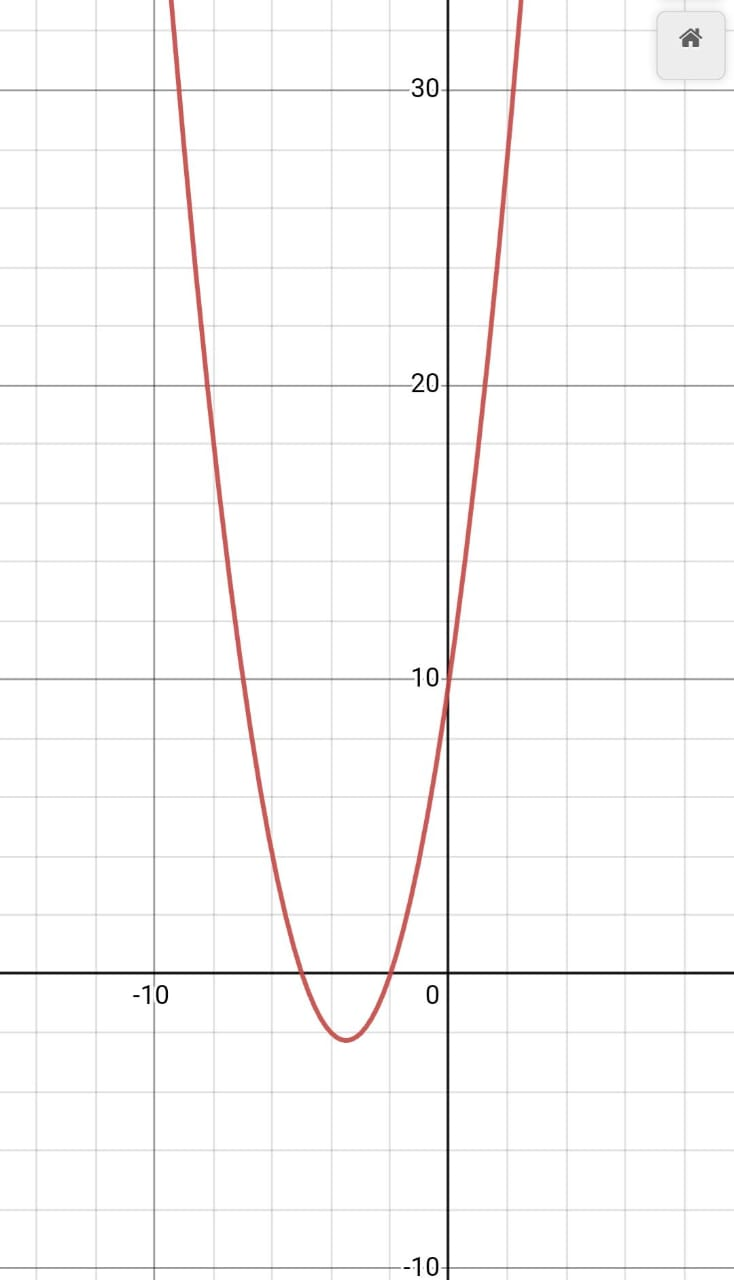
\includegraphics[width=4.5cm]{imagen/hola.jpg}
\caption{Gráfica de una ecuación cuadrática.}
\label{fig:grafica}
\end{figure}
\\

 \subsection{Descripción del problema}
Dada una ecuación cuadrática regresar los valores de las raíces en caso de que estén sobre el conjunto de los números reales, en caso contrario indicar que la solución está en el conjunto de los números complejos.

\subsection{Diseño de solución}
El discriminante que definiremos como $ D = b^2 - 4ac$ determina la naturaleza de las raíces:
\begin{itemize}
    \item Si $D > 0$, las raíces son números reales distintos.
    \item Si $D = 0$, las raíces son números reales iguales.
    \item Si $D < 0$, las raíces son números complejos conjugados.
\end{itemize}

\subsection{Desarrollo de solución}

\begin{javaCode}

        System.out.print("Coeficiente a: ");
        double a = input.nextDouble();
        System.out.print("Coeficiente b: ");
        double b = input.nextDouble();
        System.out.print("Coeficiente c: ");
        double c = input.nextDouble();
        double discriminante = b * b - 4 * a * c;
        if (discriminante > 0) {
            double raiz1 = (-b + Math.sqrt(discriminante)) / (2 * a);
            double raiz2 = (-b - Math.sqrt(discriminante)) / (2 * a);
            System.out.println("Las raices son numeros reales distintos:");
            System.out.println("Raiz 1: " + raiz1);
            System.out.println("Raiz 2: " + raiz2);
        } else if (discriminante == 0) {
            double raiz = -b / (2 * a);
            System.out.println("Las raices son numeros reales iguales:");
            System.out.println("Raiz: " + raiz);
        } else {
            System.out.println("Las raices son numeros complejos conjugados.");
        }

\end{javaCode}

\subsection{Depuración y pruebas}

\begin{table}[!ht]
\label{T:equipos}
\begin{center}
\begin{tabular}{| c | c | c | c | c |}
\hline
\textbf{$a$} & \textbf{$b$} & \textbf{$c$} & \textbf{$x_1$} & \textbf{$x_2$} \\
\hline
1 & 1 & 1 & Complejos & Complejos \\
1 & 10 & 25 & -5 & -5 \\
3 & -5 & 2 & 1 & 2/3\\
6 & -36 & 0 & 6 & 0 \\
1 & 2 & 3 & Complejos & Complejos \\
\hline
\end{tabular}
\caption{Tabla de corridas.}
\end{center}
\end{table}

En el cuadro 1 se muestra una tabla de pruebas con diferentes valores en $a$, $b$ y $c$ en las tres primeras columnas, y el valor de las raíces arrojadas por el programa, en las dos últimas columnas.